\begin{figure}[ht]
    \centering
    \subcaptionbox{Vorticity $\zeta$\label{fig:zeta_ppm}%
    }[\linewidth]{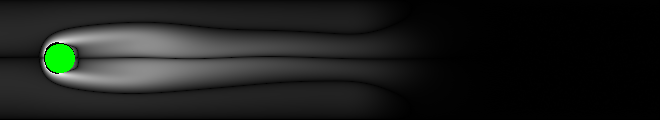
\includegraphics[width=\linewidth,natwidth=660,natheight=120]{Ch20Research/figures/output_zeta.png}
    }
    
    \subcaptionbox{Stream Function $\psi$\label{fig:psi_ppm}%
    }[\linewidth]{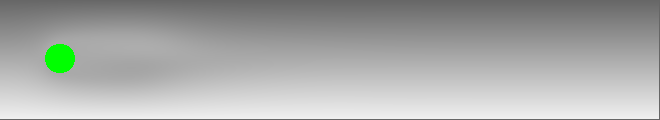
\includegraphics[width=\linewidth,natwidth=660,natheight=120]{Ch20Research/figures/output_psi.png}
    }
    
    \subcaptionbox{Pressure $p$\label{fig:pressure_ppm}%
    }[\linewidth]{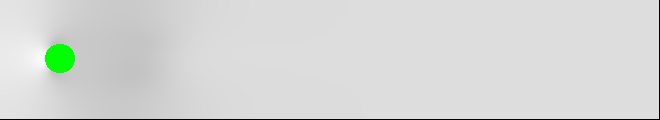
\includegraphics[width=\linewidth,natwidth=660,natheight=120]{Ch20Research/figures/output_pressure.png}
    }
    \caption{Examples of the three outputs available from the original visualization.}%\\These all visualize the output of a modified ACA coursework running for 10 seconds on the provided input data.
    %  all visualizing the same state.
    \label{fig:ppms}
\end{figure}